
\begin{figure*}[t]
  \centering
  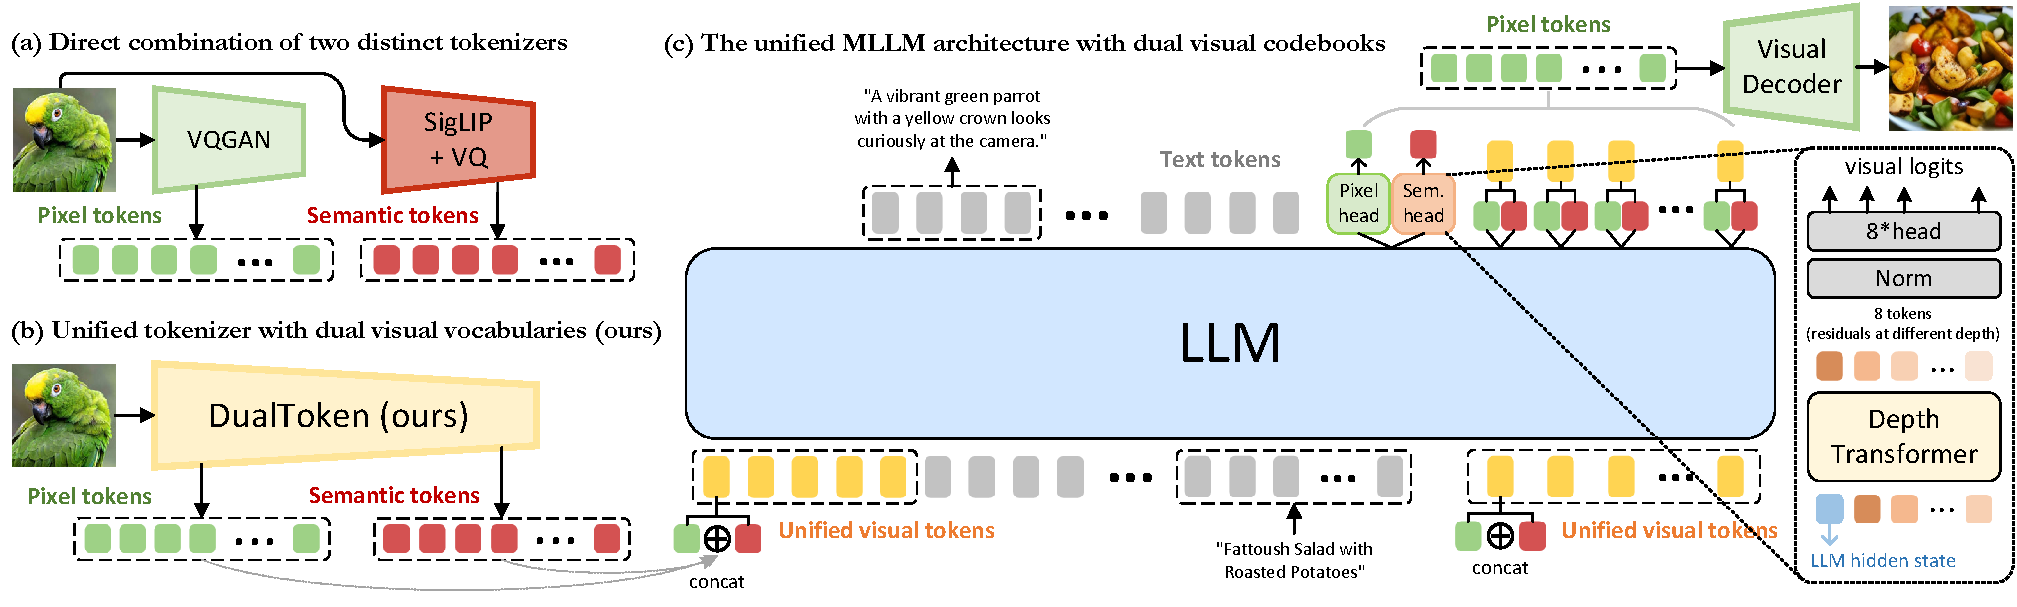
\includegraphics[width=\textwidth]{imgs/frameworks-v4.pdf}
  \caption{
      % \textbf{
      % (Left) Comparing directly 
      % An overview of our framework utilizing dual visual codebooks for unified visual understanding and generation.
      % }
      \textbf{(a) Direct combination of two heterogeneous tokenizer.} Baseline method~\citep{huang2025illume+} that directly uses VQGAN and CLIP-based encoder to separately acquire high-level (semantic) and low-level (pixel) visual codebooks.
      \textbf{(b) Our unified tokenizer with dual codebook.} We decoupling high-level and low-level visual codebooks within a unified vision tokenizer. The image is converted into low-level visual appearance tokens (green) and text-aligned semantic tokens (red).
      \textbf{(c) Architecture for unifying generation and understanding task.} % To model both textual and visual modality within the autoregressive paradigm, the pixel and semantic visual tokens are concatenated along their embedding dimension to form unified visual tokens (yellow). These unified visual tokens are then concatenated with text tokens to construct a multimodal token sequence.
      % The high-level and low-level visual tokens are predicted by independent visual heads (Pixel head and Semantic head).
      In image generation task, the generated low-level tokens are decoded by the visual decoder to reconstruct the visual content.
  }
  \label{fig:frameworks}
  % \vspace{-20pt}
\end{figure*}
